\documentclass[../report.tex]{subfiles}
\begin{document}   

\subsection{Introduction}

With over 100 million monthly listeners \cite{musicoomph} and a steadily increasing user base, there is no doubt that podcasts are a greatly enriching source of information and entertainment for a large variety of individuals.

Although they are highly valuable, it can be difficult to find podcasts that are of interest to a particular user amidst the 1 million \cite{musicoomph} that are already available.
Thus, podcast streaming services (such as UltraCast) have been created, to provide a centralised place for exploring and discovering new podcasts that are valuable to the listener.

However, all of the web based podcast streaming services available lack many important features, and their interfaces leave much to be desired. For example, there is no streaming service that allows the user to bookmark certain parts of a podcast, nor take notes at certain timestamps. It is even difficult to find a service that allows the listener to change the playback speed of the podcast.

UltraCast combines all of the most important features together into a single package with a web-based podcast streaming service.

UltraCast differentiates itself from competitors by allowing users to:
\begin{itemize}
    \item Follow friends to see what they have been listening to
    \item Create \textit{streams} of podcasts to find interesting podcasts
    \item Create bookmarks inside podcast episodes
    \item Monitor episode and podcast play metrics
\end{itemize}

\subsection{Project Requirements}
The minimum project requirements from the specifications are:
\begin{itemize}
    \item Listeners must be able to search for podcasts that interest them by keywords, resulting in a list of matching podcast titles, where the total number of subscriptions on the UltraCast platform (function described later) for each podcast is shown next to the title
    \item Listeners must be able to select a podcast show from returned search results to view its full details, including its title, description, any author details that exist, as well as a list of episodes for the show 
    \item Listeners must be able to play a selected episode within a podcast show, and once that episode starts being played, the listener must be able to also clearly see this episode marked as \textit{played}
    \item Listeners must be able to subscribe or unsubscribe from a podcast show         Listeners must be able to see the latest episode available for each show that they subscribed to in a \textit{Podcast Subscription Preview} panel
    \item Listeners must be notified by the platform when a new episode for a show  they are subscribed appears
    \item Listeners must be able to see a history of the podcast episodes that they have played, sorted in order from most recently played to least recently played
    \item UltraCast must be able to recommend new podcast shows to a listener based on at least information about the podcast shows they are subscribed to, podcast episodes they have recently played, and their past podcast searches
\end{itemize}
%
The following additional requirements have also been implemented:
\begin{itemize}
    \item Listeners should be able to follow their \textit{friends} and view the podcasts that their \textit{friends} have recently listened to
    \item Listeners should be able to create \textit{streams} based off search queries that they can use to find interesting podcasts
    \item Listeners should be able to add bookmarks with a name and description to podcast episodes as they listen to them
    \item Content creators should be able to create and upload podcasts and podcast episodes
    \item Content creators should be able to monitor analytics of their uploaded podcasts related to their listeners
\end{itemize}

Requirements testing has been performed and the results can be found in \cref{app:requirements_testing}.
UltraCast fulfils all requirements.

\newpage

\subsection{System Architecture}

The high-level system architecture can be seen in \cref{fig:system_architecture}.
The end users, podcast listeners and content creators, connect to the presentation layer 
which is powered by a ReactJS application. ReactJS was selected as the framework for the 
frontend application primarily due to it being a mature and world leading framework\cite{react} as well
as due to previous experience with the framework.\\

Flask, a python based micro-framework\cite{flask}, was used for the web-server, due to its ease of use which allowed
for rapid development. The React application communicates with Flask web-server through a GraphQL API: 
a scalable alternative to the popular REST API\cite{graphql}. The Flask web-server also contains a
recommendation service which drives recommendation functionality described in 
\cref{ssec:recommendations_and_following,ssec:system}. The Flask web-server uploads static files 
(episode audio and podcast covers) to a static file storage server while
the urls for these static files along with all other data is stored in MongoDB. MongoDB, a NoSQL database, 
was selected to store meta-data due to its scalability\cite{MongoDB2020}. MongoDB could not be hosted on
CSE so was hosted on AWS EC2 instead, see Table \ref{tab:third_party} for reason. As a result the Flask web-server
needed to be on the remote server as well to improve performance as described in \cref{ssec:backend_challenges}.
Algolia, a search engine service\cite{algolia}, was used to maximise search performance and reduce development time.

\begin{figure}[ht] 
    \centering
    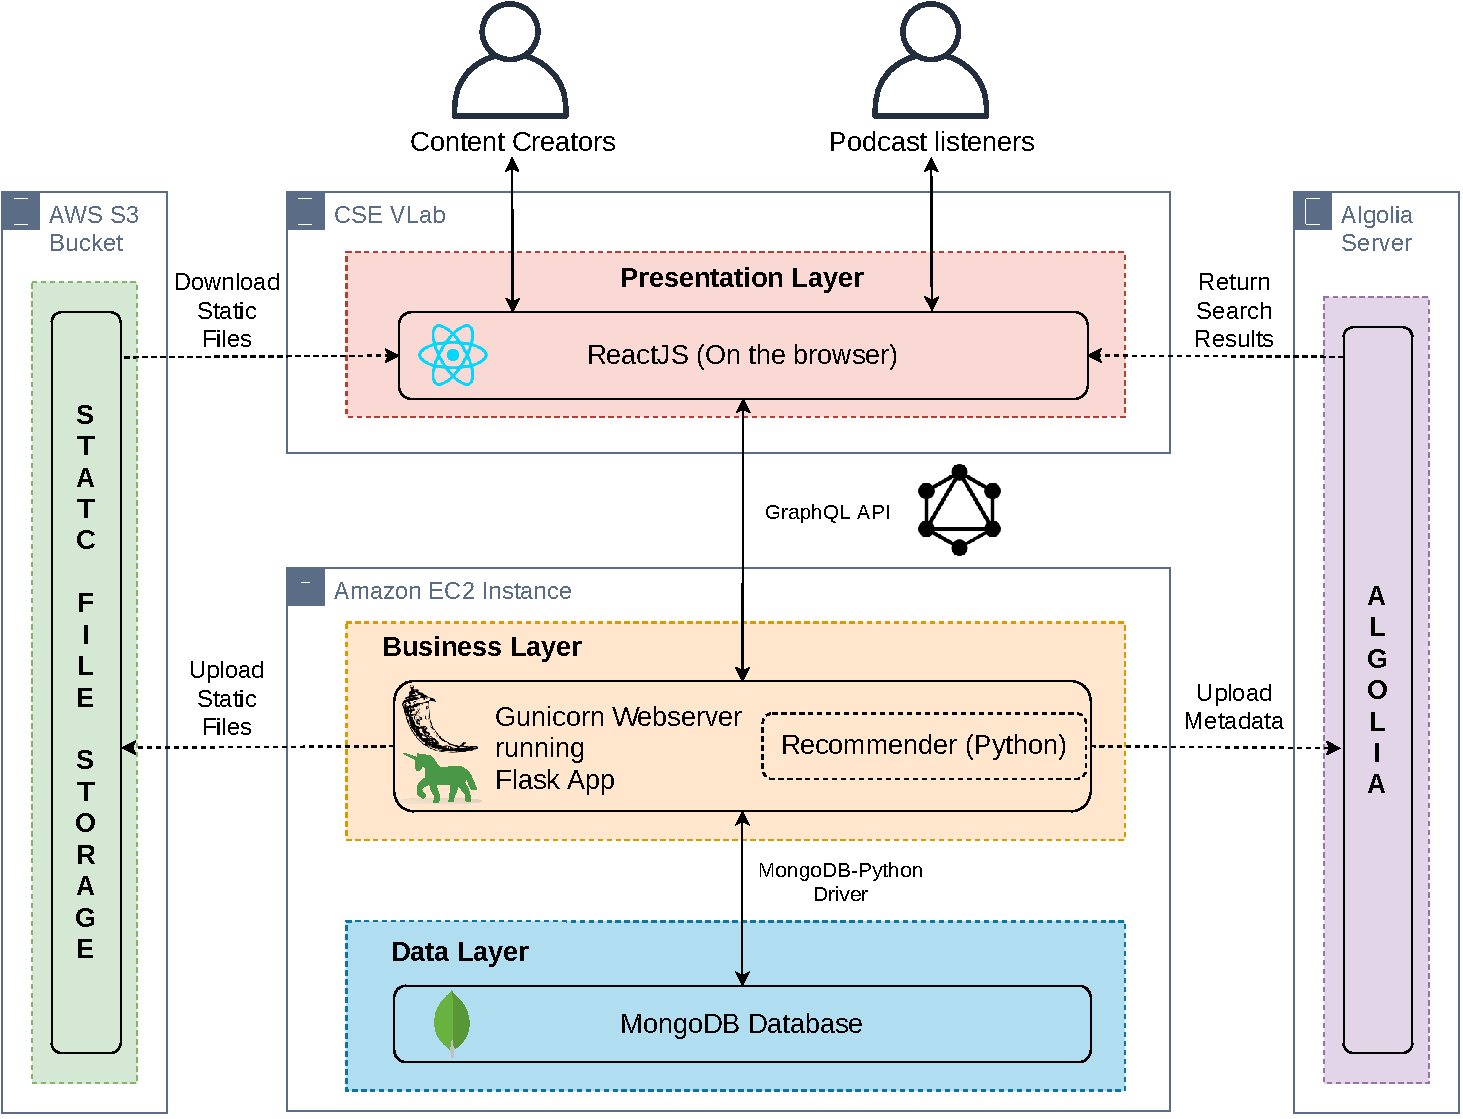
\includegraphics[width=16cm]{resources/SystemArchitecture}
    \caption{UltraCast System Architecture}
    \label{fig:system_architecture} 
\end{figure}

\newpage

\subsubsection{Third Party Components}

The third party components which had a notable impact on the functionality
of UltraCast are shown in \cref{tab:third_party}. This is not an exhaustive
list of all the libraries and system libraries in UltraCast but rather a list
of components which were notable and impacted functionality.

\begin{longtable}[c]{|l|l|l|}
    \caption{Third Party Components}
    \label{tab:third_party}\\
    \hline
    \rowcolor[HTML]{E2E2E2} 
    \textbf{Name} & \textbf{Component Type}                                                         & \textbf{Reason For Use}                                                                                              \\ \hline
    \endfirsthead
    %
    \endhead
    %
    AWS S3        & Cloud: Static File Storage                                                      & \begin{tabular}[c]{@{}l@{}}Exceeded CSE server storage limits. \\ \textgreater 80GB of test data\end{tabular}        \\ \hline
    AWS EC2       & Cloud: Remote Server                                                            & \begin{tabular}[c]{@{}l@{}l@{}}High scalability \\ MongoDB not supported on Debian 6 \\ (Linux environment on the VLab machine)\end{tabular} \\ \hline
    Algolia       & SaaS: Search Engine                                                             & \begin{tabular}[c]{@{}l@{}}Excellent search performance \\ Avoids building search engine from scratch \end{tabular}                                                                            \\ \hline
    React         & Frontend Framework                                                              & Bootstrap and provide basic functionality                                                                            \\ \hline
    Flask         & Micro Framework                                                                 & Bootstrap and provide basic functionality                                                                            \\ \hline
    Graphene      & Python GraphQL Library                                                          & Standard library                                                                                                     \\ \hline
    MongoEngine   & \begin{tabular}[c]{@{}l@{}}Python object data mapper\\ for MongoDB\end{tabular} & Standard library                                                                                                     \\ \hline
    Pandas        & Python data Library                                                             & Standard library                                                                                                     \\ \hline
    NumPy         & Python maths Library                                                            & Standard library                                                                                                     \\ \hline
\end{longtable}

\end{document}
